\documentclass{ximera}
\graphicspath{  %% When looking for images,
{./}            %% look here first,
{./pictures/}   %% then look for a pictures folder,
{../pictures/}  %% which may be a directory up.
{../../pictures/}  %% which may be a directory up.
{../../../pictures/}  %% which may be a directory up.
{../../../../pictures/}  %% which may be a directory up.
}

\usepackage{listings}
%\usepackage{circuitikz}
\usepackage{xcolor}
\usepackage{amsmath,amsthm}
\usepackage{subcaption}
\usepackage{graphicx}
\usepackage{tikz}
%\usepackage{tikz-3dplot}
\usepackage{amsfonts}
%\usepackage{mdframed} % For framing content
%\usepackage{tikz-cd}

  \renewcommand{\vector}[1]{\left\langle #1\right\rangle}
  \newcommand{\arrowvec}[1]{{\overset{\rightharpoonup}{#1}}}
  \newcommand{\ro}{\texttt{R}}%% row operation
  \newcommand{\dotp}{\bullet}%% dot product
  \renewcommand{\l}{\ell}
  \let\defaultAnswerFormat\answerFormatBoxed
  \usetikzlibrary{calc,bending}
  \tikzset{>=stealth}
  




%make a maroon color
\definecolor{maroon}{RGB}{128,0,0}
%make a dark blue color
\definecolor{darkblue}{RGB}{0,0,139}
%define the color fourier0 to be the maroon color
\definecolor{fourier0}{RGB}{128,0,0}
%define the color fourier1 to be the dark blue color
\definecolor{fourier1}{RGB}{0,0,139}
%define the color fourier 1t to be the light blue color
\definecolor{fourier1t}{RGB}{173,216,230}
%define the color fourier2 to be the dark green color
\definecolor{fourier2}{RGB}{0,100,0}
%define teh color fourier2t to be the light green color
\definecolor{fourier2t}{RGB}{144,238,144}
%define the color fourier3 to be the dark purple color
\definecolor{fourier3}{RGB}{128,0,128}
%define the color fourier3t to be the light purple color
\definecolor{fourier3t}{RGB}{221,160,221}
%define the color fourier0t to be the red color
\definecolor{fourier0t}{RGB}{255,0,0}
%define the color fourier4 to be the orange color
\definecolor{fourier4}{RGB}{255,165,0}
%define the color fourier4t to be the darker orange color
\definecolor{fourier4t}{RGB}{255,215,0}
%define the color fourier5 to be the yellow color
\definecolor{fourier5}{RGB}{255,255,0}
%define the color fourier5t to be the darker yellow color
\definecolor{fourier5t}{RGB}{255,255,100}
%define the color fourier6 to be the green color
\definecolor{fourier6}{RGB}{0,128,0}
%define the color fourier6t to be the darker green color
\definecolor{fourier6t}{RGB}{0,255,0}

%New commands for this doc for errors in copying
\newcommand{\eigenvar}{\lambda}
%\newcommand{\vect}[1]{\mathbf{#1}}
\renewcommand{\th}{^{\text{th}}}
\newcommand{\st}{^{\text{st}}}
\newcommand{\nd}{^{\text{nd}}}
\newcommand{\rd}{^{\text{rd}}}
\newcommand{\paren}[1]{\left(#1\right)}
\newcommand{\abs}[1]{\left|#1\right|}
\newcommand{\R}{\mathbb{R}}
\newcommand{\C}{\mathbb{C}}
\newcommand{\Hilb}{\mathbb{H}}
\newcommand{\qq}[1]{\text{#1}}
\newcommand{\Z}{\mathbb{Z}}
\newcommand{\N}{\mathbb{N}}
\newcommand{\q}[1]{\text{``#1''}}
%\newcommand{\mat}[1]{\begin{bmatrix}#1\end{bmatrix}}
\newcommand{\rref}{\text{reduced row echelon form}}
\newcommand{\ef}{\text{echelon form}}
\newcommand{\ohm}{\Omega}
\newcommand{\volt}{\text{V}}
\newcommand{\amp}{\text{A}}
\newcommand{\Seq}{\textbf{Seq}}
\newcommand{\Poly}{\textbf{P}}
\renewcommand{\quad}{\text{    }}
\newcommand{\roweq}{\simeq}
\newcommand{\rowop}{\simeq}
\newcommand{\rowswap}{\leftrightarrow}
\newcommand{\Mat}{\textbf{M}}
\newcommand{\Func}{\textbf{Func}}
\newcommand{\Hw}{\textbf{Hamming weight}}
\newcommand{\Hd}{\textbf{Hamming distance}}
\newcommand{\rank}{\text{rank}}
\newcommand{\longvect}[1]{\overrightarrow{#1}}
% Define the circled command
\newcommand{\circled}[1]{%
  \tikz[baseline=(char.base)]{
    \node[shape=circle,draw,inner sep=2pt,red,fill=red!20,text=black] (char) {#1};}%
}

% Define custom command \strikeh that just puts red text on the 2nd argument
\newcommand{\strikeh}[2]{\textcolor{red}{#2}}

% Define custom command \strikev that just puts red text on the 2nd argument
\newcommand{\strikev}[2]{\textcolor{red}{#2}}

%more new commands for this doc for errors in copying
\newcommand{\SI}{\text{SI}}
\newcommand{\kg}{\text{kg}}
\newcommand{\m}{\text{m}}
\newcommand{\s}{\text{s}}
\newcommand{\norm}[1]{\left\|#1\right\|}
\newcommand{\col}{\text{col}}
\newcommand{\sspan}{\text{span}}
\newcommand{\proj}{\text{proj}}
\newcommand{\set}[1]{\left\{#1\right\}}
\newcommand{\degC}{^\circ\text{C}}
\newcommand{\centroid}[1]{\overline{#1}}
\newcommand{\dotprod}{\boldsymbol{\cdot}}
%\newcommand{\coord}[1]{\begin{bmatrix}#1\end{bmatrix}}
\newcommand{\iprod}[1]{\langle #1 \rangle}
\newcommand{\adjoint}{^{*}}
\newcommand{\conjugate}[1]{\overline{#1}}
\newcommand{\eigenvarA}{\lambda}
\newcommand{\eigenvarB}{\mu}
\newcommand{\orth}{\perp}
\newcommand{\bigbracket}[1]{\left[#1\right]}
\newcommand{\textiff}{\text{ if and only if }}
\newcommand{\adj}{\text{adj}}
\newcommand{\ijth}{\emph{ij}^\text{th}}
\newcommand{\minor}[2]{M_{#2}}
\newcommand{\cofactor}{\text{C}}
\newcommand{\shift}{\textbf{shift}}
\newcommand{\startmat}[1]{
  \left[\begin{array}{#1}
}
\newcommand{\stopmat}{\end{array}\right]}
%a command to give a name to explorations and hints and theorems
\newcommand{\name}[1]{\begin{centering}\textbf{#1}\end{centering}}
\newcommand{\vect}[1]{\vec{#1}}
\newcommand{\dfn}[1]{\textbf{#1}}
\newcommand{\transpose}{\mathsf{T}}
\newcommand{\mtlb}[2][black]{\texttt{\textcolor{#1}{#2}}}
\newcommand{\RR}{\mathbb{R}} % Real numbers
\newcommand{\id}{\text{id}}
\newcommand{\coord}[1]{\langle#1\rangle}
\newcommand{\RREF}{\text{RREF}}
\newcommand{\Null}{\text{Null}}
\newcommand{\Nullity}{\text{Nullity}}
\newcommand{\Rank}{\text{Rank}}
\newcommand{\Col}{\text{Col}}
\newcommand{\Ef}{\text{EF}}
\newcommand{\boxprod}[3]{\abs{(#1\times#2)\cdot#3}}

\author{Zack Reed}
%borrowed from selinger linear algebra
\title{Lines Revisited}
\begin{document}
\begin{abstract}

\end{abstract}
\maketitle

\section*{More Explicit Definitions of Lines}

We conclude this section by revisiting two fundamental subspaces of $\RR^n$, lines and planes. These particular formulations are particularly useful when using linear algebra to examine physical systems described in $\RR^3$, which is crucial for engineering and the physical sciences. 

Both characterizations relate to the dot product, and so these provide a fitting conclusion to the chapter. 

First, a brief review. 

\subsection*{Lines and Planes as Subspaces}
  
We have examined lines and planes much in this course already, and have primarily described them in terms of span. Specifically, lines through the origin are $1$-dimensional subspaces of $\RR^n$, defined by the span of a single vector $\vec{u}_1$. 

Planes through the origin, similarly, are $2$-dimensional subspaces of $\RR^n$ defined as the span of two vectors $\vec{u}_1$ and $\vec{u}_2$.

We now leverage the ideas of unit directional vectors, parallel vectors, and normal vectors, to more explicitly reconceptualize key features of lines and planes (and then hyperplanes as well).

\subsection*{Lines in $\RR^n$ as Directional Spans}

We can build from the idea of lines as $1$-dimensional spans to better align the more familiar characterizations of lines from previous courses, and to set the stage for fairly effective characterizations of planes and hyperplanes as well.

\begin{exploration}\label{init:paramline2d}

  In courses such as algebra and calculus, lines were typically represented in ``standard form'', conveying an explicit relationships between the coordinates $(x,y)$ of any point on the line as

  $$y=mx+b,$$

  where it was understood that $m$ represented the ``slope'' and $b$ represented where the line intersected with the vertical axis. 

  For instance, consider the line $y=-\frac{3}{2}x+\frac{9}{2}$, in the following figure. 


  \begin{center}
    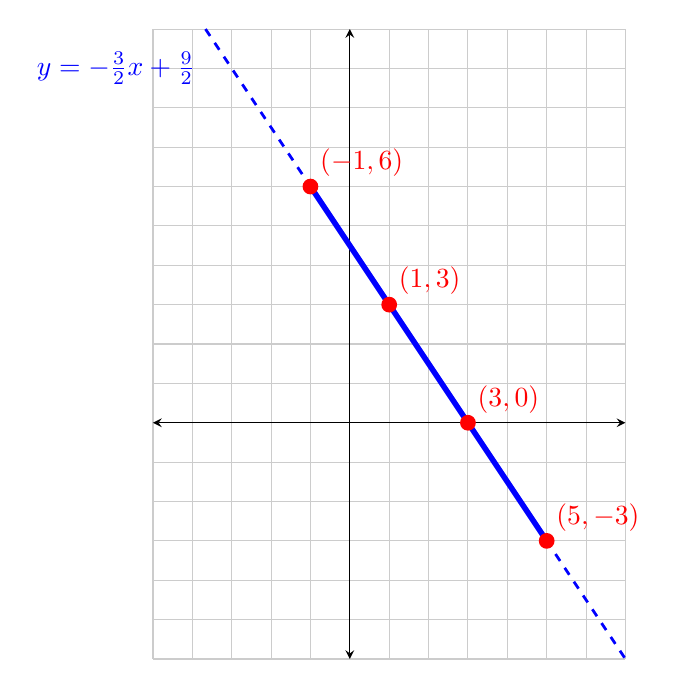
\begin{tikzpicture}[scale=0.5]
    \draw[thin,gray!40] (-5,-6) grid (7,10);
      \draw[<->] (-5,0)--(7,0);
      \draw[<->] (0,-6)--(0,10);
       
    \draw[line width=2pt,blue](-1,6)--(5,-3) ;
     
    \draw[line width=1pt,blue, dashed](-11/3,10)node[below=5mm, left=0mm]{$y=-\frac{3}{2}x+\frac{9}{2}$}--(7,-6) ;
     
    \fill[red] (-1,6) node[above right]{$(-1,6)$} circle (0.2cm);
    \fill[red] (1,3) node[above right]{$(1,3)$} circle (0.2cm);
    \fill[red] (3,0) node[above right]{$(3,0)$} circle (0.2cm);
    \fill[red] (5,-3) node[above right]{$(5,-3)$} circle (0.2cm);
     \end{tikzpicture}
    \end{center}

  The locations in red on the line are all explicitly found according to the standard formula, and are at times computed in tables such as the following:

  $$\begin{array}{|c|c|c|} 
  \hline t& x & y\\
  \hline 0 & -1 & 6\\
  \hline 1 & 1 & 3 \\
  \hline 2 & 3& 0\\
  \hline 3 & 5& -3\\
  \hline
  \end{array}$$

  From a linear algebra perspective, a line represents the locations of vector heads, so each line gives us a collection of vectors that are all related, as seen in the following figure:

  \begin{center}
    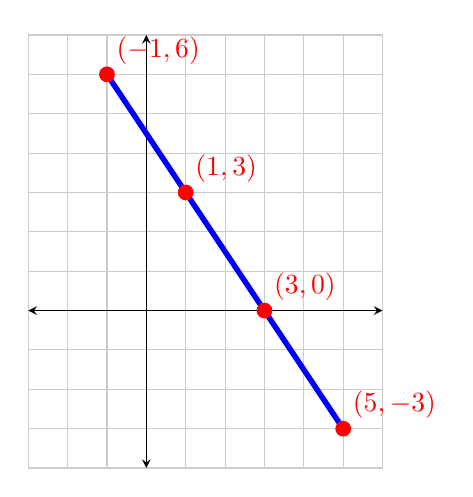
\begin{tikzpicture}[scale=0.5]
    \draw[thin,gray!40] (-3,-4) grid (6,7);
      \draw[<->] (-3,0)--(6,0);
      \draw[<->] (0,-4)--(0,7);
      \draw[line width=2pt,blue](-1,6)--(5,-3) ;
      \fill[red] (-1,6) node[above right]{$(-1,6)$} circle (0.2cm);
      \fill[red] (1,3) node[above right]{$(1,3)$} circle (0.2cm);
      \fill[red] (3,0) node[above right]{$(3,0)$} circle (0.2cm);
      \fill[red] (5,-3) node[above right]{$(5,-3)$} circle (0.2cm);
     \end{tikzpicture}
     \quad
     \quad
     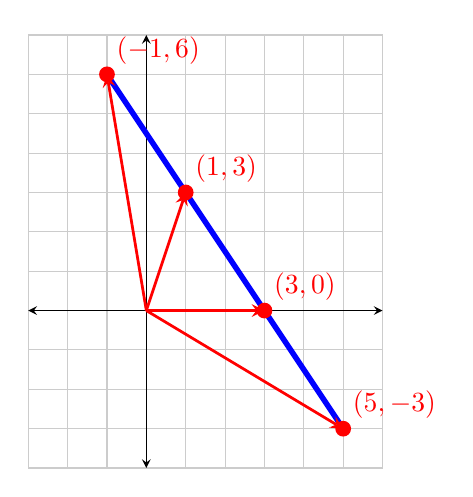
\begin{tikzpicture}[scale=0.5]
    \draw[thin,gray!40] (-3,-4) grid (6,7);
      \draw[<->] (-3,0)--(6,0);
      \draw[<->] (0,-4)--(0,7);
      \draw[line width=2pt,blue](-1,6)--(5,-3) ;
      \draw[line width=1pt,red,-stealth](0,0)--(-1,6) ;
      \draw[line width=1pt,red,-stealth](0,0)--(1,3) ;
      \draw[line width=1pt,red,-stealth](0,0)--(3,0) ;
      \draw[line width=1pt,red,-stealth](0,0)--(5,-3) ;
      \fill[red] (-1,6) node[above right]{$(-1,6)$} circle (0.2cm);
      \fill[red] (1,3) node[above right]{$(1,3)$} circle (0.2cm);
      \fill[red] (3,0) node[above right]{$(3,0)$} circle (0.2cm);
      \fill[red] (5,-3) node[above right]{$(5,-3)$} circle (0.2cm);
     \end{tikzpicture}
  \end{center}

  From a linear algebra perspective, it becomes less important to think about a relationship between variables such as $x$ and $y$, particularly because this would become very complex when dealing with thousands of variables all at once. Rather, we build on the idea of span, direction and vector addition to come up with a concise representation of lines. 
  
  All you need to describe a line is to pick a \emph{starting point} $\vec{p}$ and a \emph{direction} $\vec{d}$. From there, you create any point on the line by scaling the direction vector and using vector addition on the chosen point $\vec{p}$. Let's use this to re-write the expression $y=-\frac{3}{2}x+\frac{9}{2}$ in vector format.

  \begin{solution}
    First, let's pick a point on the line, kind of as a center point, from which we build the rest of the line. 

    Which vector we choose doesn't quite matter at this stage, so let's go with $\vec{p}=\begin{bmatrix}
      1\\3
    \end{bmatrix}$ as our starting point.

    From there, let's find the direction vector that determines movement along the line. 

    In the following diagram, we start at the vector $\vec{p}$, and then move to the next vector in our example, $\begin{bmatrix}
      3\\0
    \end{bmatrix}$. 

    \begin{center}
      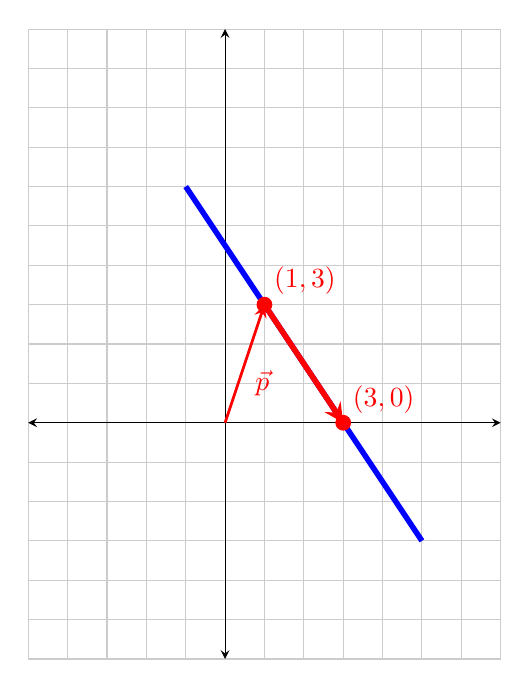
\begin{tikzpicture}[scale=0.5]
      \draw[thin,gray!40] (-5,-6) grid (7,10);
        \draw[<->] (-5,0)--(7,0);
        \draw[<->] (0,-6)--(0,10);
         
      \draw[line width=2pt,blue](-1,6)--(5,-3) ;
       
      \draw[line width=1pt,blue, dashed](-11/3,10);%node[below=5mm, left=0mm]{$y=-\frac{3}{2}x+\frac{9}{2}$}--(7,-6) ;
       
      %\fill[red] (-1,6) node[above right]{$(-1,6)$} circle (0.2cm);
      \fill[red] (1,3) node[above right]{$(1,3)$} circle (0.2cm);
      \fill[red] (3,0) node[above right]{$(3,0)$} circle (0.2cm);
      %\fill[red] (5,-3) node[above right]{$(5,-3)$} circle (0.2cm);

      \draw[line width=1pt,red,-stealth](0,0)node[above=5mm, right=2.5mm]{$\vec{p}$}--(1,3);
      \draw[line width=2pt,red,-stealth](1,3)--(3,0) ;
       \end{tikzpicture}
      \end{center}

      The vector taking us from $\vec{p}$ to $\begin{bmatrix}
        3\\0
      \end{bmatrix}$ is $d=\begin{bmatrix}
        \answer{2}\\\answer{-3}
      \end{bmatrix}$. (Hint: Think about the slope of the line).

      Now, we can describe any other vector on the line by vector addition $\vec{p}+\lambda \vec{d}$, where $\lambda$ is the scalar multiple. (Note: $\vec{d}$ will typically be a unit direction vector, but it doesn't have to be, and here it will make the next problem simpler if it remains as is).

    Armed with $\vec{p}$ and $\vec{d}$, write the remaining sample points on the line in vector format:

    \begin{center}
      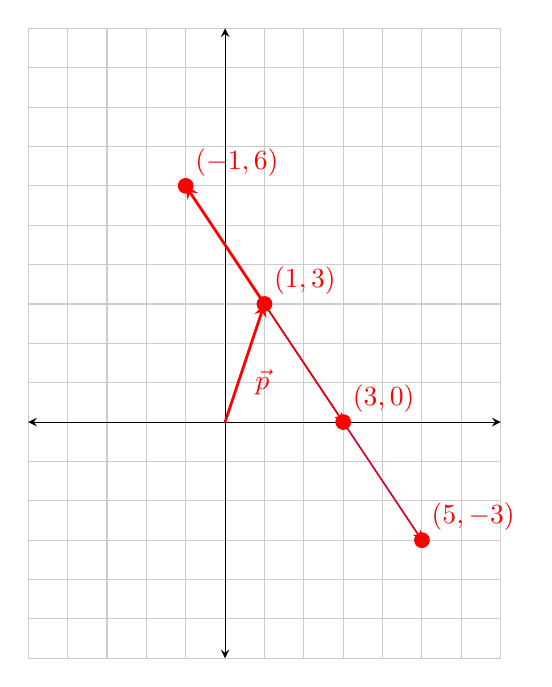
\begin{tikzpicture}[scale=0.5]
      \draw[thin,gray!40] (-5,-6) grid (7,10);
        \draw[<->] (-5,0)--(7,0);
        \draw[<->] (0,-6)--(0,10);
         
      \draw[line width=.5pt,blue](-1,6)--(5,-3) ;
       
      \draw[line width=.5pt,blue, dashed](-11/3,10);%node[below=5mm, left=0mm]{$y=-\frac{3}{2}x+\frac{9}{2}$}--(7,-6) ;
       
      \fill[red] (-1,6) node[above right]{$(-1,6)$} circle (0.2cm);
      \fill[red] (1,3) node[above right]{$(1,3)$} circle (0.2cm);
      \fill[red] (3,0) node[above right]{$(3,0)$} circle (0.2cm);
      \fill[red] (5,-3) node[above right]{$(5,-3)$} circle (0.2cm);

      \draw[line width=1pt,red,-stealth](0,0)node[above=5mm, right=2.5mm]{$\vec{p}$}--(1,3);
      \draw[line width=1pt,red,-stealth](1,3)--(-1,6) ;
      \draw[line width=.5pt,red,-stealth](1,3)--(3,0) ;
      \draw[line width=.5pt,red,-stealth](1,3)--(5,-3) ;
       \end{tikzpicture}
      \end{center}

  \end{solution}

  We reach $(-1,6)$ by the sum $\vec{p}+\answer{-1}\vec{d}$, $(1,3)$ by the sum $\vec{p}+\answer{0}\vec{d}$, $(3,0)$ by the sum $\vec{p}+\answer{1}\vec{d}$, and $(5,-3)$ by the sum $\vec{p}+\answer{2}\vec{d}$.

  While these were straightforward scalars, the process is the same for any point on the line, we simply find the correct amound by which to scale $\vec{d}$ after shifting away from $\vec{0}$ by $\vec{p}$.

\end{exploration}

This brings us to a new definition of a line:

\begin{definition}
  A line in $\RR^n$ is the set of all vectors of the form 

  $$\vec{p}+\lambda \vec{d},$$

  where $\lambda$ is a scalar and $\vec{p}$ and $\vec{d}$ are vectors in $\RR^n$.
\end{definition}

Notice that this definition scales very well to large vector spaces, since we don't need to deal with thousands and thousands of variables, and can instead focus on the key vectors $\vec{p}$ and $\vec{d}$.
 
\begin{example}\name{A line from a point and a direction vector}\label{ex:line-point-and-direction-vector}

  Write a vector equation for the line which contains the point
  $P = (2,0,3)$ and has unit direction vector $\vec{d}$ in the direction of 
  $\begin{bmatrix}1\\2\\1\end{bmatrix}$.



Solution:

  The position vector of the point $P$ is
  $\vec{p}=\begin{bmatrix}2\\0\\3\end{bmatrix}$. 

  The unit direction vector is in the direction of $\begin{bmatrix}1\\2\\1\end{bmatrix}$, but is a unit vector. Hence, we find the magnitude $\norm{\begin{bmatrix}1\\2\\1\end{bmatrix}}=\answer{\sqrt{6}}$ (Note: Enter the exact number, not a decimal).
  
  Rounding the direction vector to two decimal places, we get the equation 
  $\vec{q}= \vec{p} + \lambda\,\vec{d}$, which we can write as
  \begin{equation*}
    \begin{bmatrix} x \\ y \\ z \end{bmatrix}
    = \begin{bmatrix} \answer{2} \\ \answer{0} \\ \answer{3} \end{bmatrix}
    + \lambda \begin{bmatrix} \answer[tolerance=.01]{.41} \\ \answer[tolerance=.01]{.82} \\ \answer[tolerance=.01]{.41} \end{bmatrix}.
  \end{equation*}
\end{example}.

There are many ways to express the equation of a line, we will tend to use the vector equation, which can also be expressed generally in component form as 

\begin{equation*}
  \begin{bmatrix} x_1 \\ x_2 \\ \vdots \\ x_n \end{bmatrix}
  = \begin{bmatrix} p_1 \\ p_2 \\ \vdots \\ p_n \end{bmatrix}
  + \lambda \begin{bmatrix} d_1 \\ d_2 \\ \vdots \\ d_n \end{bmatrix},
\end{equation*}

Notice that the vector equation of a line is not unique. In fact,
there are infinitely many vector equations for the same line. For
example, we can replace the parameter $\lambda$ with another parameter, say $t$ (which is often used) or 
$3s$ or $1-r$. We can also choose any vector $\vec{p}$ on the line, and any direction vector $\vec{d}$ (though we tend to like unit direction vectors).

\begin{example}\name{Determine whether a point is on a line}\label{ex:point-on-line}

  Determine whether the point $P=(5,8,4)$ is on the line $L$ given by
  the vector equation
  \begin{equation*}
    \begin{bmatrix} x \\ y \\ z \end{bmatrix}
    = \begin{bmatrix} 1 \\ 2 \\ 1 \end{bmatrix}
    + t \begin{bmatrix} 2 \\ 3 \\ 1 \end{bmatrix}.
  \end{equation*}
\end{example}

\begin{solution}
  There are actually two solutions to this problem, and one will reveal a connection back to the dot product that we will then exploit further to similarly characterize planes in productive ways.

  First, the point $P$ is on the line $L$ if and only if there exists some
  $t\in\R$ such that
  \begin{equation*}
    \begin{bmatrix} 1 \\ 2 \\ 1 \end{bmatrix}
    + t \begin{bmatrix} 2 \\ 3 \\ 1 \end{bmatrix}
    = \begin{bmatrix} 5 \\ 8 \\ 4 \end{bmatrix}.
  \end{equation*}
  Subtracting $\begin{bmatrix}1,2,1\end{bmatrix}$ from both sides of the equation, this is
  equivalent to
  \begin{equation*}
    t \begin{bmatrix} 2 \\ 3 \\ 1 \end{bmatrix}
    = \begin{bmatrix} 4 \\ 6 \\ 3 \end{bmatrix}.
  \end{equation*}

  This vector equation is only satisfied if the following three equations are satisfied.

  \begin{equation*}
    \begin{array}{c@{~}c@{~}l}
      \answer{2}t &=& \answer{4}, \\
      \answer{3}t &=& \answer{6}, \\
      \answer{t} &=& \answer{3}.
    \end{array}
  \end{equation*}

  This is a system of three linear equations in one variable, and we
  quickly see that it is \wordChoice{
    \choice{consistent}
    \choice[correct]{inconsistent}}. Therefore, the point $P$ \wordChoice{
      \choice{does}
      \choice[correct]{does not}}
  lie on the line $L$.

\end{solution}

This next solution will also set up a more general theme on which we will capitalize to describe planes and hyperplanes.

\begin{solution}

  As a second solution, we can use orthogonality to our advantage. Since we know the direction vector, if we find a vector orthogonal to $\vec{d}$ (call the orthogonal vector $\vec{n}$), then after displacement by $\vec{p}$ any vector on the line will also be orthogonal to $\vec{n}$.

  For reference, consider the line from the beginning of the section:

  \begin{center}
    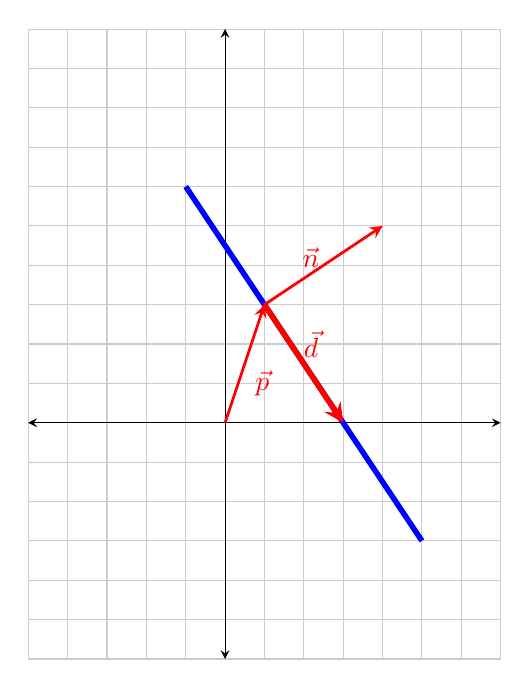
\begin{tikzpicture}[scale=0.5]
    \draw[thin,gray!40] (-5,-6) grid (7,10);
      \draw[<->] (-5,0)--(7,0);
      \draw[<->] (0,-6)--(0,10);
       
    \draw[line width=2pt,blue](-1,6)--(5,-3) ;
     
    \draw[line width=1pt,blue, dashed](-11/3,10);%node[below=5mm, left=0mm]{$y=-\frac{3}{2}x+\frac{9}{2}$}--(7,-6) ;
     
    %\fill[red] (-1,6) node[above right]{$(-1,6)$} circle (0.2cm);
    %\fill[red] (1,3) node[above right]{$(1,3)$} circle (0.2cm);
    %\fill[red] (3,0) node[above right]{$(3,0)$} circle (0.2cm);
    %\fill[red] (5,-3) node[above right]{$(5,-3)$} circle (0.2cm);

    \draw[line width=1pt,red,-stealth](0,0)node[above=5mm, right=2.5mm]{$\vec{p}$}--(1,3);
    \draw[line width=2pt,red,-stealth](1,3)node[below=5mm, right=3.5mm]{$\vec{d}$}--(3,0) ;
    \draw[line width=1pt, red, -stealth](1,3)node[above=6mm,right=3.5mm]{$\vec{n}$}--(4,5);
     \end{tikzpicture}
    \end{center}

  The direction vector $\vec{d}=\begin{bmatrix}
    2\\-3
  \end{bmatrix}$ is orthogonal to the vector $\vec{n}=\begin{bmatrix}
    3\\2
  \end{bmatrix}$ (note that $2\times 3+(-3)\times 2=0$).

  Because the dot product repsects scaling, anything in $\mbox{span}(\vec{d})$ will also be orthogonal to $\vec{n}$. So, if we take any point on the line, undo the displacement by $\vec{p}$ and then check for orthogonality with $\vec{n}$, we should also get a zero dot product.

  In our current example, there is actually a whole plane of vectors orthogonal to our line 

  \begin{equation*}
    \begin{bmatrix} 1 \\ 2 \\ 1 \end{bmatrix}
    + t \begin{bmatrix} 2 \\ 3 \\ 1 \end{bmatrix}
    = \begin{bmatrix} 5 \\ 8 \\ 4 \end{bmatrix}.
  \end{equation*}

  (you'll see why in the next section). So we have plenty of vector $\vec{n}$ to choose from. One such vector is $\vec{n}=\begin{bmatrix}
    -3\\1\\3
  \end{bmatrix}$. 
  
  To check, calculate 

  $$\vec{d}\cdot \vec{n}=\answer{-6}+\answer{3}+\answer{3}=0.$$

  Thus, after we undo the displacement by $\vec{p}=\begin{bmatrix}
    1\\2\\1
  \end{bmatrix}$, the vector $\begin{bmatrix}
    5\\8\\4
  \end{bmatrix}-\begin{bmatrix}
    1\\2\\1
  \end{bmatrix}$ should be orthogonal to $\vec{n}$.

  To check, we calculate

  $$\left(\begin{bmatrix}
    5\\8\\4
  \end{bmatrix}-\begin{bmatrix}
    1\\2\\1
  \end{bmatrix}\right)\cdot \begin{bmatrix}
    -3\\1\\3
  \end{bmatrix}=\begin{bmatrix}
    \answer{4}\\\answer{6}\\\answer{3}
  \end{bmatrix}\cdot \begin{bmatrix}
    -3\\1\\3
  \end{bmatrix}=\answer{-12}+\answer{6}+\answer{9}=\answer{3}.$$

  Thus, again we see that $\begin{bmatrix}
    5\\8\\4
  \end{bmatrix}$ is not on the line.

  This solution, in addition to setting up representations of planes and hyperplanes in $\RR^n$, also involves \emph{centering} data back to $\vec{0}$ to make some useful calculations. This is a strategy we have enacted before, and will be important again moving forward.


\end{solution}

\begin{example}\name{Determine whether two lines intersect}\label{ex:lines-intersect}

  Determine whether the lines
  \begin{equation*}
    \begin{bmatrix} x \\ y \\ z \end{bmatrix}
    = \begin{bmatrix} 3 \\ 1 \\ 0 \end{bmatrix}
    + t \begin{bmatrix} 2 \\ 0 \\ 1 \end{bmatrix}
    \quad\mbox{and}\quad
    \begin{bmatrix} x \\ y \\ z \end{bmatrix}
    = \begin{bmatrix} 1 \\ -1 \\ 5 \end{bmatrix}
    + s \begin{bmatrix} 2 \\ 1 \\ -2 \end{bmatrix}
  \end{equation*}
  intersect. If yes, find the point of intersection.%
  \index{intersection!of two lines}
\end{example}




\begin{solution}
  One of the well-known properties of $\RR^n$ is that two lines that are not parallel are guaranteed to meet!This is something you would have seen back in high school geometry,but comes up from time to time when in popular discourse folks compare this property to the geometry of spheres, where some parallel lines meet.

  Hence, to find whether the lines meet, we need to determine if they are paralle. Luckily, all this entails is a comparison of the direction vectors $\begin{bmatrix} 2 \\ 0 \\ 1 \end{bmatrix}$ and $\begin{bmatrix} 2 \\ 1 \\ -2 \end{bmatrix}$. If they are parallel, then the lines will not meet (unless they are the same line), and if they are not parallel then the lines are guaranteed to meet.

  Being parallel means pointing in the exact same direction, so to compare directions, we convert the two vectors to unit vectors and take their dot product!

  The first direction vector has magnitude 
  
  $$\norm{\begin{bmatrix} 2 \\ 0 \\ 1 \end{bmatrix}}=\answer{\sqrt{5}},$$
  
  so the first unit direction vector, we'll call it $\vec{d}_1$, is approximately 

  $$\vec{d_1}\approx\begin{bmatrix}
    \answer[tolerance=.01]{.89}\\\answer[tolerance=.01]{0}\\\answer[tolerance=.01]{.45}
  \end{bmatrix}.$$

  Similarly, the second direction vector, we'll call it $\vec{d}_2$, is approximately

  $$\vec{d_2}\approx\begin{bmatrix}
    \answer[tolerance=.01]{.67}\\\answer[tolerance=.01]{.33}\\\answer[tolerance=.01]{-.67}
  \end{bmatrix}.$$  

  Using MATLAB for a quick dot product, we get 

  $$\vec{d_1}\cdot\vec{d_2}=\answer{.29}.$$

  Therefore, the lines do indeed intersect, since their direction vectors are not parallel!
  
  The two lines intersect at $t,s$ in $R$ such
  that
  \begin{equation*}
    \begin{bmatrix} 3 \\ 1 \\ 0 \end{bmatrix}
    + t \begin{bmatrix} 2 \\ 0 \\ 1 \end{bmatrix}
    = \begin{bmatrix} 1 \\ -1 \\ 5 \end{bmatrix}
    + s \begin{bmatrix} 2 \\ 1 \\ -2 \end{bmatrix}.
  \end{equation*}
  Bringing $s$ to the left-hand side, and subtracting $\begin{bmatrix}3,1,0\end{bmatrix}$
  from both sides of the equation, this is equivalent to
  \begin{equation*}
    t \begin{bmatrix} 2 \\ 0 \\ 1 \end{bmatrix}
    - s \begin{bmatrix} 2 \\ 1 \\ -2 \end{bmatrix}
    = \begin{bmatrix} -2 \\ -2 \\ 5 \end{bmatrix}.
  \end{equation*}
  This is a system of 3 linear equations in 2 variables. 
  
  The
  augmented matrix of the system is
  \begin{equation*}
    \begin{bmatrix}
      2 & -2 & -2 \\
      0 & -1 & -2 \\
      1 & 2 & 5   \\
    \end{bmatrix}.
  \end{equation*}
  This system has {\rref}
  \begin{equation*}
    \begin{bmatrix}
      1 & 0 & 1 \\
      0 & 1 & 2 \\
      0 & 0 & 0 \\
    \end{bmatrix},
  \end{equation*}
  and has the unique solution $t=\answer{1}$ and $s=\answer{2}$.
  
 Plugging in $t$ or $s$ into their respective equations, we get the point of intersection is
  \begin{equation*}
    \begin{bmatrix} 3 \\ 1 \\ 0 \end{bmatrix}
    + 1 \begin{bmatrix} 2 \\ 0 \\ 1 \end{bmatrix}
    = \begin{bmatrix} 5 \\ 1 \\ 1 \end{bmatrix}.
  \end{equation*}
\end{solution}


Similar to our use of the dot product to determine whether the liens were parallel, we can also use the dot product to find the angle between two intersecting
lines. This is simply the smallest angle between (any of) their
direction vectors. The only subtlety here is that if $\vec{u}$ is a
direction vector for a line, then so is $-\vec{u}$, and thus we will
find pairs of complementary angles. We will take the smaller of the
two angles.

\begin{center} 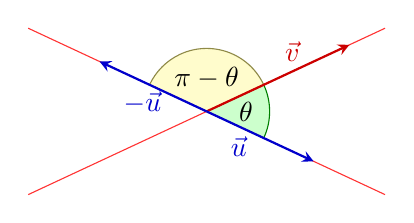
\begin{tikzpicture}
    \filldraw[fill=green!20,draw=green!50!black] (0,0) -- (-25:8mm)
    arc (-25:25:8mm) -- cycle;
    \filldraw[fill=yellow!20,draw=yellow!50!black] (0,0) -- (25:8mm)
    arc (25:155:8mm) -- cycle;
    \node at (0:5mm) {$\theta$};
    \node at (90:4.2mm) {$\pi-\theta$};
    \draw[red!80](25:-2.5) -- (25:2.5);
    \draw[red!80](-25:-2.5) -- (-25:2.5);
    \draw[->,thick,red!80!black](0,0) -- node[above,pos=0.6]{$\vec{v}$} (25:2);
    \draw[->,thick,blue!80!black](0,0) -- node[below,pos=0.3]{$\vec{u}$} (-25:1.5);
    \draw[->,thick,blue!80!black](0,0) -- node[below,pos=0.6]{$-\vec{u}$} (155:1.5);
  \end{tikzpicture}
\end{center}

\begin{example}\name{Find the angle between two lines}\label{ex:angle-between-two-lines}

  Find the angle between the two lines%
  \index{line!angle between}%
  \index{angle!between two lines}
  \begin{equation*}
    L_1:  \;
    \begin{bmatrix} x \\ y \\ z \end{bmatrix}
    = \begin{bmatrix} 1 \\ 2 \\ 0 \end{bmatrix}
    + t \begin{bmatrix} -1 \\ 1 \\ 2 \end{bmatrix}
  \end{equation*}
  and
  \begin{equation*}
    L_2: \;
    \begin{bmatrix} x \\ y \\ z \end{bmatrix}
    = \begin{bmatrix} 0 \\ 3 \\ 2 \end{bmatrix}
    + s \begin{bmatrix} 2 \\ 1 \\ -1 \end{bmatrix}.
  \end{equation*}
\end{example}



\begin{solution}
  The direction vectors are
  \begin{equation*}
    \vec{u}=\begin{bmatrix} -1 \\ 1 \\ 2 \end{bmatrix}
    \quad\mbox{and}\quad
    \vec{v}=\begin{bmatrix} 2 \\ 1 \\ -1 \end{bmatrix}.
  \end{equation*}

  In this case we don't need to convert to unit vectors, as we can directly use the definition of the dot product to generate the desired angle. 
  
  Recall that one formluation of the dot product is 
  
  $$\vec{u}\cdot\vec{v}=\norm{\vec{u}}\norm{\vec{v}}\cos(\theta).$$
  
  Hence, we can solve for the cosine of the angle measure (or $\theta$) as necessary. 
  
  We calculate
  \begin{equation*}
    \cos\theta =
    \frac{\vec{u}\dotprod\vec{v}}{\norm{\vec{u}}\norm{\vec{v}}} = \answer{-1/2},
  \end{equation*}
  which between $\theta=0$ and $\theta=\pi$ gives $\theta=\answer{\frac{2\pi}{3}}$ (give an exact answer in terms of $\pi$).  
  
 The complementary angle (i.e. $\pi-\theta$) is $\answer{\frac{\pi}{3}}$. We
  choose the smaller angle, and therefore conclude that the angle
  between the two lines is $\answer{\frac{\pi}{3}}$.
\end{solution}


\end{document}